\documentclass[]{scrartcl} 

\usepackage[T1]{fontenc}
\usepackage{lmodern}
\usepackage[utf8]{inputenc}
%\usepackage[ngerman]{babel}

\usepackage{amsfonts,amssymb,amsmath,amsthm}
\usepackage{graphicx}  
\usepackage{marginnote}
%\usepackage[usenames,dvipsnames]{color}
\usepackage[dvipsnames]{xcolor}
\usepackage{natbib}
\usepackage{authblk}
\usepackage{enumitem}
\usepackage{tabularx}
\usepackage{subfigure}
\usepackage{mathtools}
\usepackage[noend]{algorithmic}
\usepackage{algorithm}

\newtheorem{theorem}{Theorem}[section]
\newtheorem{acknowledgment}[theorem]{Acknowledgment}
\newtheorem{corollary}[theorem]{Corollary}
\newtheorem{definition}[theorem]{Definition}
\newtheorem{remark}[theorem]{Remark}
\newtheorem{lemma}[theorem]{Lemma}
\newtheorem{problem}[theorem]{Problem}
\newtheorem{proposition}[theorem]{Proposition}
\newtheorem{observation}[theorem]{Observation}
\newtheorem{example}[theorem]{Example}



\newcommand{\argmax}[1]{\underset{#1}{\operatorname{arg\,\max}}}
\newcommand{\bigOsymb}{\ensuremath{\mathcal{O}}}
\newcommand{\bigO}[1]{\ensuremath{\mathcal{O}\left(#1\right)}}
\newcommand{\eps}{\texorpdfstring{\ensuremath{\epsilon}}{epsilon}}
\newcommand{\norm}[1]{\lvert\lvert #1 \rvert\rvert}

\newcommand{\lp}[1]{\marginpar{\textcolor{red!80!black}{\footnotesize MW: #1}}}
\newcommand{\cf}[1]{\marginpar{\textcolor{green!20!white}{\footnotesize LS: #1}}}
\newcommand{\kknote}[1]{\marginpar{\textcolor{magenta}{\footnotesize KK: #1}}}
\newcommand{\jf}[1]{\marginpar{\textcolor{green!50!black}{\footnotesize TD: #1}}}
\newcommand{\bs}[1]{\marginpar{\textcolor{pink}{\footnotesize BS: #1}}}
\newcommand{\ms}[1]{\marginpar{\textcolor{blue}{\footnotesize MS: #1}}}
\newcommand{\todo}[1]{\textcolor{red}{ #1}}

\newcommand{\dmk}{, \ldots ,}

\DeclarePairedDelimiter{\ceil}{\lceil}{\rceil}


\DeclareMathOperator*{\vmin}{vmin}
\DeclareMathOperator*{\vmax}{vmax}
\DeclareMathOperator*{\twomax}{2-\!\max}
\newcommand{\colvec}[2][.9]{%
  \scalebox{#1}{$\left(\renewcommand*{\arraystretch}{0.75}\begin{array}{@{}c@{}}#2\end{array}\right)$}}%

\newcommand{\argmin}[1]{\underset{#1}{\operatorname{arg\,\min}}}

\newcommand{\E}{\ensuremath{\mathcal{E}}}
\newcommand{\X}{\ensuremath{\mathcal{X}}}
\newcommand{\Xeff}{\ensuremath{\mathcal{X}_{E}}}
\newcommand{\Ynondom}{\ensuremath{\mathcal{Y}_{N}}}
\newcommand{\ten}{\text{TEN}}

\usepackage{tikz, pgfplots}
\usetikzlibrary{arrows, shapes.misc, chains, patterns}
\usetikzlibrary{decorations.pathreplacing}
\usepackage{xifthen}

\tikzset{
  candidat/.style={rectangle, inner sep=0pt, minimum size=0.1cm, draw=gray, fill=gray},
  nds/.style={circle, inner sep=0pt, minimum size=0.12cm, draw=black, fill=black},
  %ndns/.style={thick, draw=red, cross out, inner sep=0pt, minimum width=4pt, minimum height=4pt},
  ndns/.style={rectangle, inner sep=0pt, minimum size=0.12cm, draw=black, fill=black},
  test/.style={circle, inner sep=0pt, minimum size=0.12cm, draw=black, fill=black},
}
\pgfplotsset{compat=1.8}





\newcommand{\cmnt}[1]{\noindent {\bf[ #1 ]}}
\newcommand{\hide}[1]{}
\newcommand{\N}{\mathbb{N}}
\newcommand{\R}{\mathbb{R}}
\newcommand{\p}{\rho}
\newcommand{\Z}{\mathbb{Z}}
\newcommand{\SH}{\ensuremath{\mathcal{SH}}}
\newcommand{\tb}{\textbf}

\begin{document} 
\section{Introduction}
Here we investigate the migratary patterns of emporer penguins in the antarctic. The migration consists of huddling penguins with individuals moving from the interior to the exterior in a cycle. Penguins on the exterior are exposed to high winds and low temperatures and must make it into the interior in order to survive. Meanwhile penguins in the interior, shielded from the wind by other penguins, are at risk of overheating. The combination of these two hazards leads to a robust migratory pattern of circulating penguins. 

\section{Model Description}
\subsection{Migration of a Single Penguin}
In our simulations each penguin is given a random initial position $\textbf{r}_i(t)$ and heading $n_i(t)$. The velocity of a penguin is given by
\begin{align}
\frac{d\textbf{r}_i(t)}{dt} = \textbf{v}_i (t)
\end{align}
where $\textbf{v}_i(t)$ is the velocity of a penguin and is given by 
\begin{align}
\textbf{v}_i(t) = v_0 [\cos\theta_i(t), \sin \theta_i(t)]
\end{align}
where the instantaneous orientation of a penguin $\theta_i(t)$ is calculated on each time step and results from the sum of several vectors that include various interactions and the penguins previous heading $n_i(t)$. The heading of a penguin is a variable quantity that relaxes towards the instantaneous orientation $\theta_i(t)$, with some added noise, according to 
\begin{align}
\frac{dn_i(t)}{dt} = - \kappa  \alpha_i(t) + \eta (t)
\end{align}
where $\alpha_i(t)$ is the angle from $\theta_i(t)$ to $n_i(t)$ and $\eta (t) $ is an uncorrelated white noise given by 
\begin{align}
\langle \eta(t) \eta(t- \tau) \rangle = \sigma^2 \delta (t) 
\end{align}
where $\sigma$ is the noise intensity. The schematic in figure 1 shows the position, velocity, heading and orientation of penguin $i$.
\begin{figure}[H]
\centering
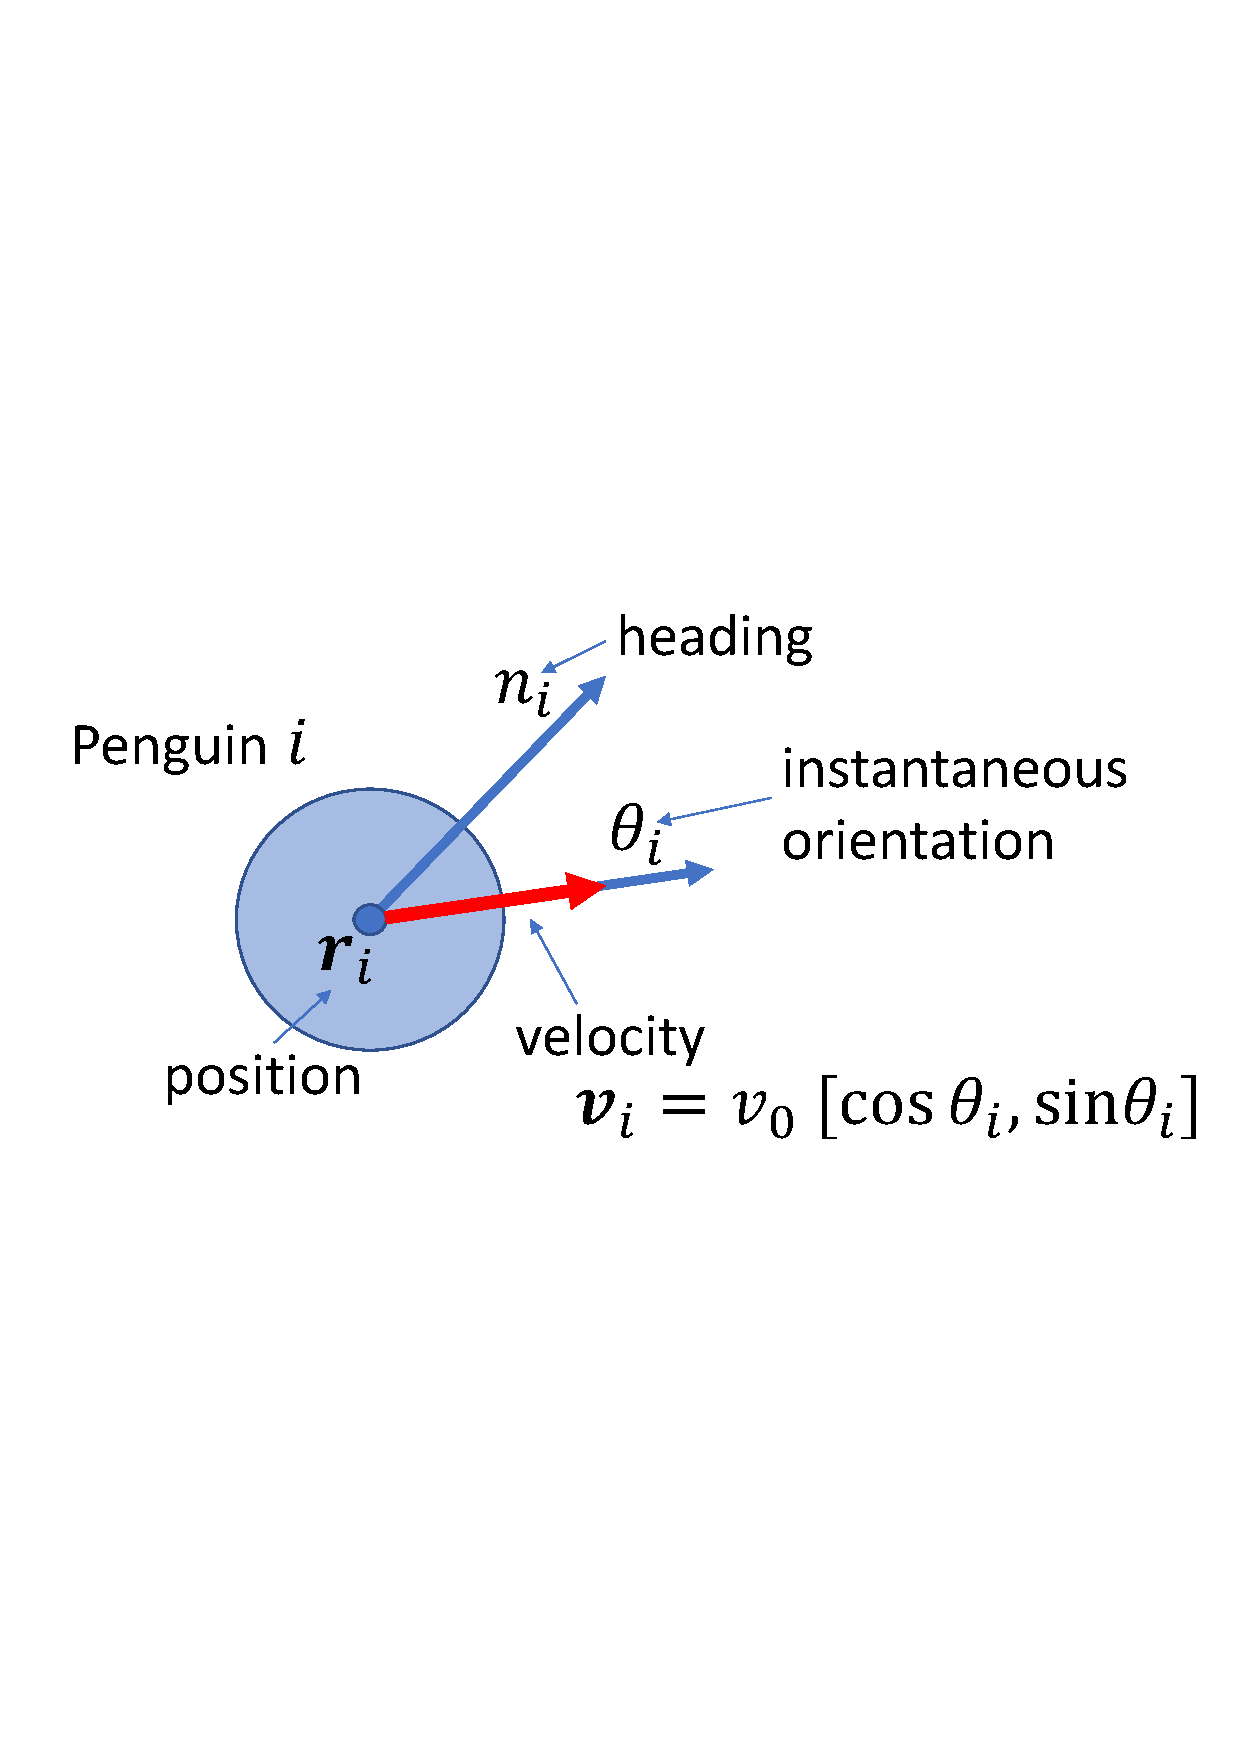
\includegraphics[width = 0.7\textwidth]{figs/fig1.pdf}
\caption{The position, velocity, heading and orientation of penguin $i$}
\end{figure}
In this model an individual penguin would perform a random walk with the mean squared displacement proportional to time where the constant of proportionality is the diffusion constant. 



\subsection{Temperature of a Single Penguin}
In our model the temperature of each penguin, $T_i$, is set to an initial value $T_i = T_{\text{init}}$. We also have temperature bounds $[T_{\min}, T_{\max}]$ and if the temperature of a penguin is outside of these bounds, we decide that the penguin is dead and we remove it from the simulation. Penguins also have a preferred temperature $T_0$ and will either climb up the temperature gradient or down the temperature gradient if their temperature is either less than or greater than this value. We write the temperature of the penguin as a first order differential equation with terms corresponding to the temperature of the external environment, wind chill, internal heat production of penguins and penguin penguin heat transfer:
\begin{align}
\frac{dT_i}{dt} = - env - wind + internal + interaction
\end{align}
The negative terms correspond to the heat loss due to thermal contact of penguins with the environment and the wind chill. The positive terms correspond to the internal heat production of penguins and to the heat exchange with neighbors. Thus, the closer the penguins are to each other, the higher the heat exchange is and so huddling penguins become warmer than isolated penguins. 

\subsection{Interaction: Collisions (Soft and Hard Interaction)}
In this model we incorporated both soft and hard repulsion between penguins. All penguins are the same size and have a radius $r$. So the minimum possible distance between two penguins without overlap is $2r$. On each time step we calculate penguin penguin distances and we find which penguins are within this distance of overlap. We find the penguins j within the repulsion range of penguin $i$ and define the repulsion of penguin $i$ from this neighbors as 
\begin{align}
\tb{F}_i (t)= \sum_j (2r - r_{ij}(t)) \frac{\tb{r}_{ij}(t)}{|\tb{r}_{ij}(t)|}
\end{align}
\begin{figure}[H]
\centering
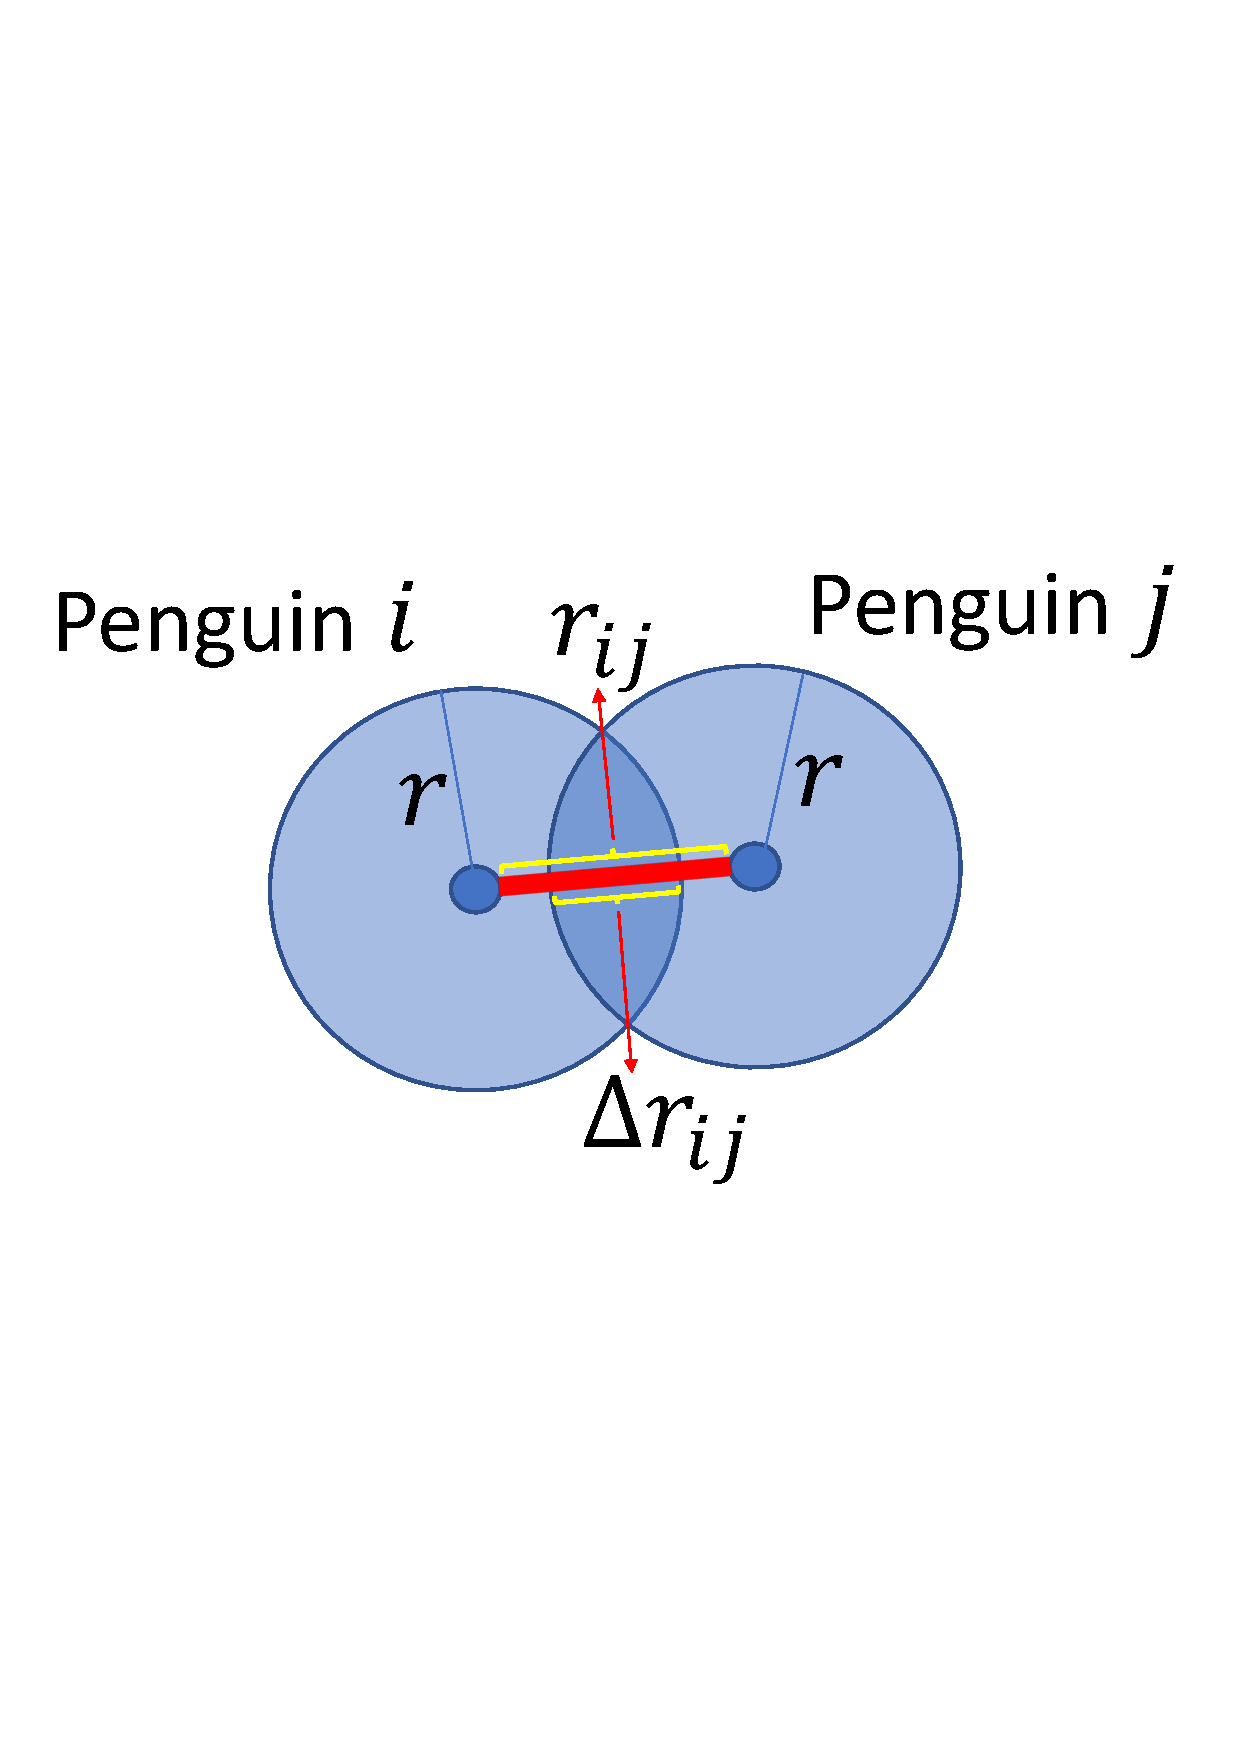
\includegraphics[width = 0.7\textwidth]{figs/fig2.pdf}
\caption{\todo{Luke wants to say something about it <3}}
\end{figure}

For hard repulsion we impose the condition that no overlaps between penguins are permitted. After a penguin is moved, if it overlaps with another penguin, we move both penguins away from one another along the line joining the centers until the overlap vanishes. This may result in introducing new overlaps with other penguins and so we repeat these steps recursively until all overlaps are removed. 

\subsection{Interaction: Temperature Gradient}
Penguins can gain heat from other penguins as long as they are close enough to one another. As such we model the heat that a penguin gives off as a gaussian centred on the penguin. Therefore the temperature $T_{i,x}$ at a distance $x$ from the penguin can be written as 
\begin{align}
T_{i,x} = T_i e^{-k x^2}
\end{align}
where $k$ defines the rate at which this temperature field diminishes. 
\begin{figure}[H]
\centering
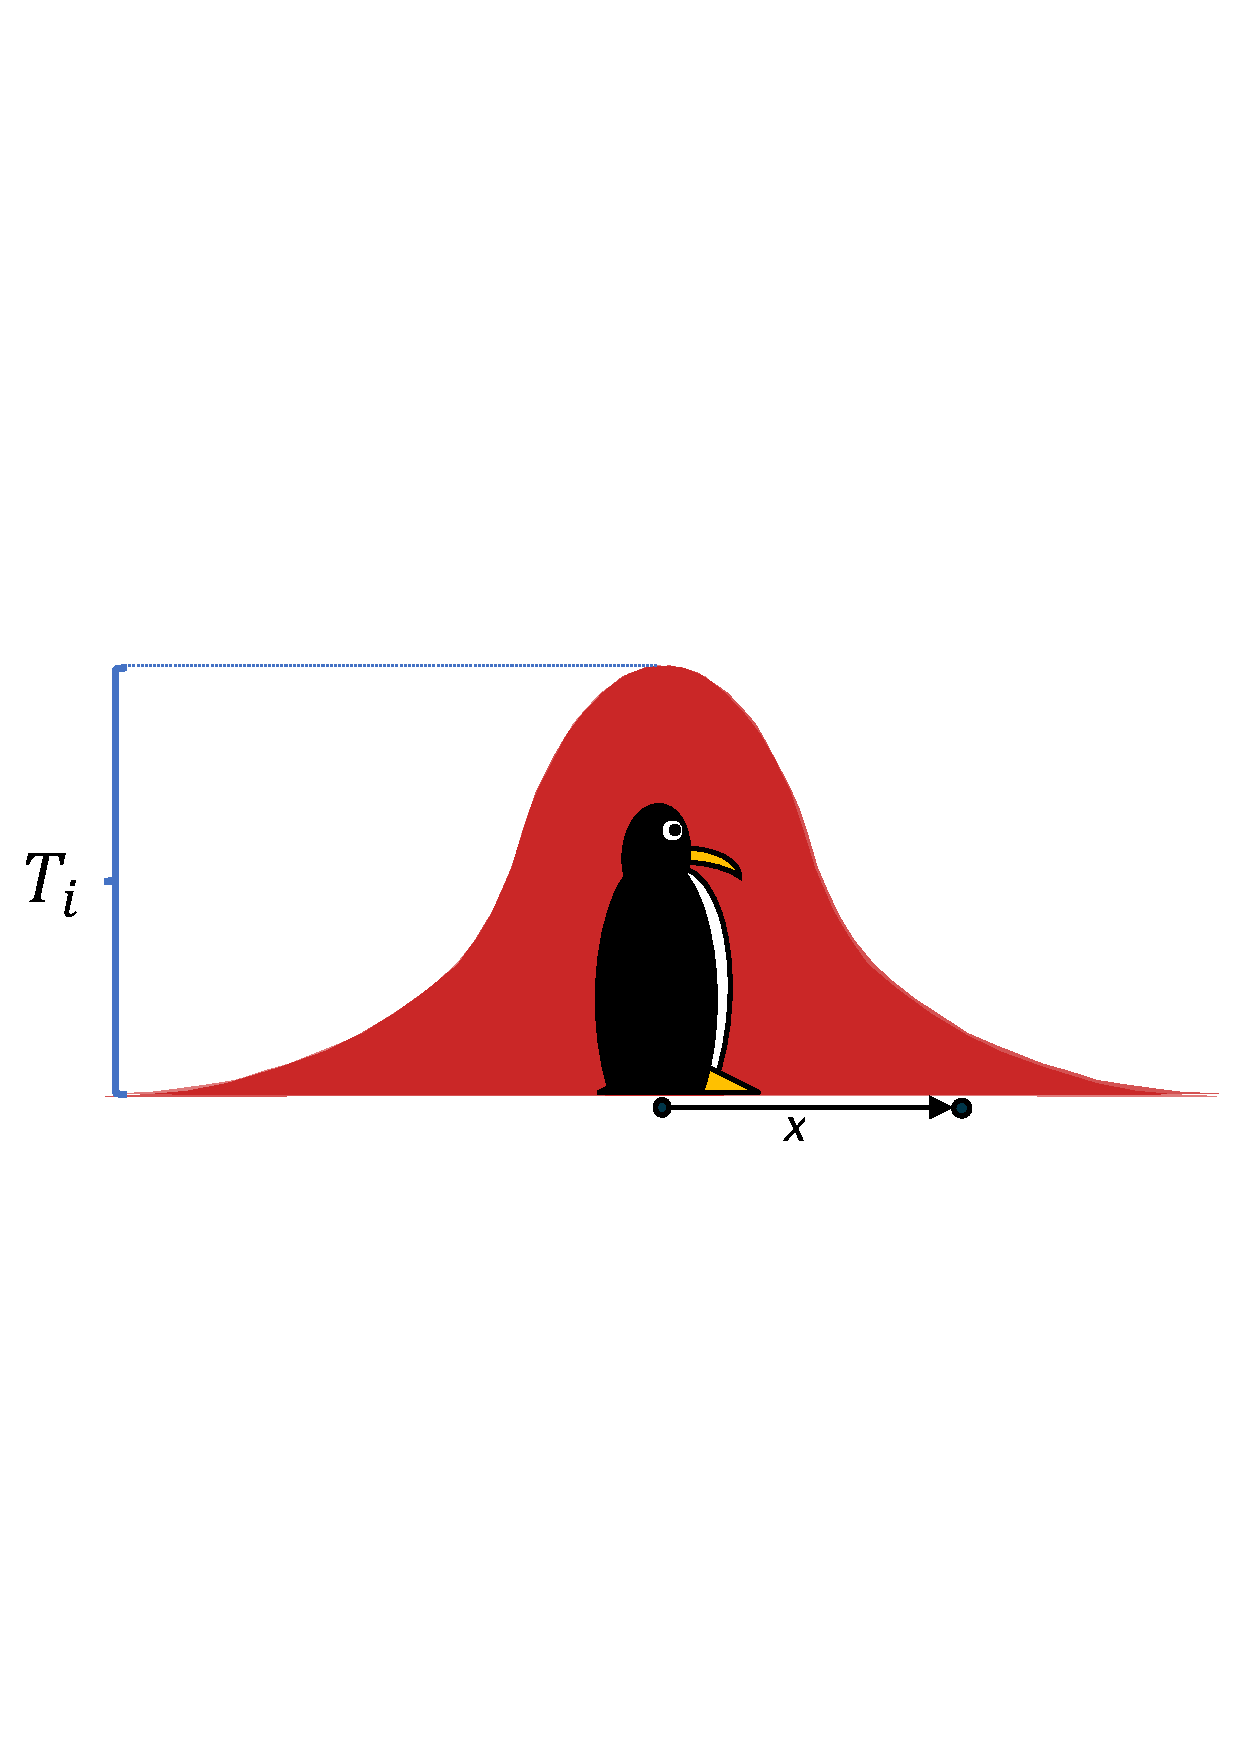
\includegraphics[width = 0.7\textwidth]{figs/fig3.pdf}
\caption{\todo{Luke wants to say something about it <3}}
\end{figure}

At time $t$ we construct vectors from penguin $i$ to all other penguins $j$ where the magnitude of these vectors is the temperature felt by penguin $i$ due to penguin $j$. Thus we can write the temperature gradient vector as 
\begin{align}
\tb{H}_i (t)= h \sum_j T_j (t) e^{-k r_{ij}(t)} \frac{\tb{r}_{ij}(t)}{|\tb{r}_{ij}(t)|}
\end{align}
where $h = 1$ if $T_i \leqslant T_0$ and $h = -1 $ if $T_i > T_0$. The purpose of this prefactor is so that the penguin will climb the temperature gradient if the temperature is less than the preferred temperature $T_0$ and will go down the gradient if it is greater than $T_0$. 

\begin{figure}[H]
\centering
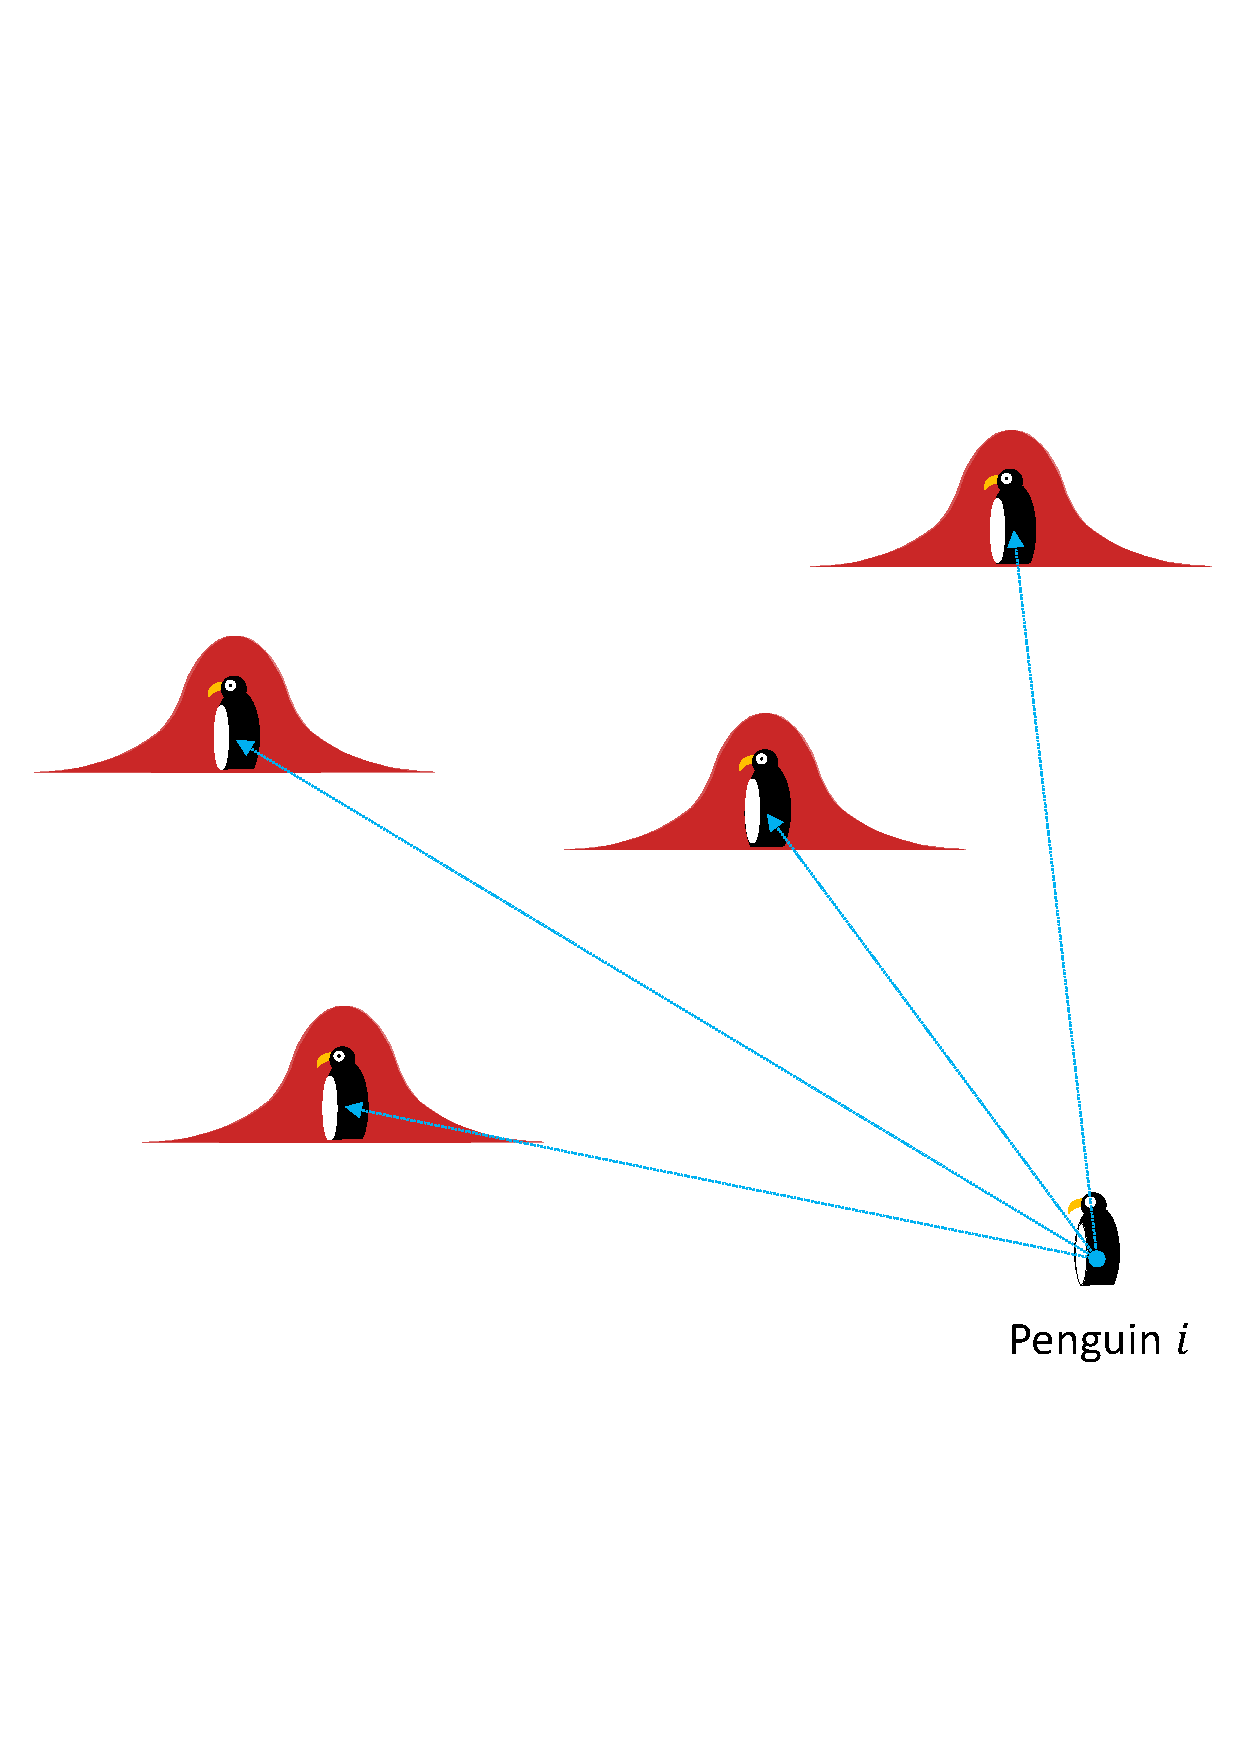
\includegraphics[width = 0.7\textwidth]{figs/fig4.pdf}
\caption{\todo{Luke wants to say something about it <3}}
\end{figure}

\subsection{Interaction: Visual}
Microscopic organisms such as bacteria may only detect one another by sampling a chemical gradient and climbing towards the regions of greater concentration. This is a mechanism by which these microscopic organisms may aggregate. Macroscopic organisms such as penguins are far more complex and have myriad ways of sensing the environment. As such we decided to incorporate a mechanism based on visual cues which would allow the penguins to aggregate in the first case. We did not want the penguins to sense one another by climbing heat gradients as we wanted the heat gradient of a penguin to be more localised and for it to decay very rapidly. 

As such at time $t$ we define this vector as 
\begin{align}
\tb{S}_i (t)= \frac{1}{N-1} \sum_j  \frac{\tb{r}_{ij}(t)}{|\tb{r}_{ij}(t)|}
\end{align}
where $N$ is the number of penguins. 

\subsection{Resultant Motion of Penguins}
FINALLY the resultant motion of a penguin is given by the instantaneous orientation $\theta_i(t)$ of penguin $i$ is calculated as follows. First of all we find the  sum of the penguins heading vector, the penguin penguin repulsion vectors (in the case that we are using soft repulsion), the temperature gradient vector and the aggregation vector: 
\begin{align}
\tb{M}_i (t)= a \tb{N}_i(t)  + b \tb{F}_i(t) + c \tb{H}_i(t) + d \tb{S}_i(t) 
\end{align}
where the prefactors $a$, $b$, $c$, $d$ weight the relative contribution of each of these vectors to the resultant vector. 
The instantaneous orientation of penguin $i$, $\theta_i(t)$, is found by finding the orientation of the resultant vector $\tb{M}_i(t)$ and the position of penguins is updated according to equation (1).

\subsection{Coding Notes}
Henriette will write the code in Python with an object oriented structure!!
no problem :)

\section{Results}
\subsection{Temperature: Ground, Wind Chill and Body Heat} 
\subsection{Migratory Patterns}

























\end{document}